\documentclass[10pt,titlepage]{article}
%\documentclass[10pt,twocolumn,titlepage]{article}
\usepackage[left=3.5cm,top=3.5cm,right=3.5cm,bottom=3.5cm]{geometry} % outter spacing settings
\usepackage{changepage}
%\usepackage{geometry} % outter spacing settings


\usepackage[utf8]{inputenc}
\usepackage[square, sort&compress, numbers]{natbib}
\usepackage{algorithm}
\usepackage{algpseudocode}
\usepackage{graphicx}
\usepackage{array}
\usepackage{comment}
\usepackage{caption}

\usepackage{enumitem}
\usepackage{hyperref}
\usepackage[all]{hypcap}
\usepackage{caption}
\usepackage{wrapfig}
\usepackage{sidecap}

\setlist{nolistsep} %reduce /item spacings


%\usepackage{cite}
\setcounter{topnumber}{2}
\setcounter{bottomnumber}{2}
\setcounter{totalnumber}{4}
\setlength{\intextsep}{5pt plus 5pt minus 5pt}

% Alter some LaTeX defaults for better treatment of Figures:
    % See p.105 of "TeX Unbound" for suggested values.
    % See pp. 199-200 of Lamport's "LaTeX" book for details.
    %   General parameters, for ALL pages:
    \renewcommand{\topfraction}{0.9}	% max fraction of floats at top
    \renewcommand{\bottomfraction}{0.8}	% max fraction of floats at bottom
    %   Parameters for TEXT pages (not float pages):
    \setcounter{topnumber}{1}
    \setcounter{bottomnumber}{1}
    \setcounter{totalnumber}{2}     % 2 may work better
    \setcounter{dbltopnumber}{1}    % for 2-column pages
    \renewcommand{\dbltopfraction}{0.9}	% fit big float above 2-col. text
    \renewcommand{\textfraction}{0.07}	% allow minimal text w. figs
    %   Parameters for FLOAT pages (not text pages):
    \renewcommand{\floatpagefraction}{0.7}	% require fuller float pages
	% N.B.: floatpagefraction MUST be less than topfraction !!
    \renewcommand{\dblfloatpagefraction}{0.7}	% require fuller float pages




\begin{document}

\begin{titlepage}
\thispagestyle{empty}
  \begin{adjustwidth}{-2cm}{-2cm}

%opening
%\title{}
%\author{Daniel L.J. Genis$^1$ \and Ey\"up S. Canlar$^2$$^,$$^3$ \and Mauro Conti$^4$ \and Bruno Crispo$^5$ \\ \and
%\\ $^1$ VU University Amsterdam, Netherlands - \texttt{dgs230@few.vu.nl}
%\\ $^2$ VU University Amsterdam, Netherlands - \texttt{escanlar@cs.vu.nl}
%\\ $^3$ Sapienza University of Rome, Italy - \texttt{canlar@di.uniroma1.it}
%\\ $^4$ University of Padua, Italy - \texttt{conti@math.unipd.it}
%\\ $^5$ University of Trento, Italy - \texttt{crispo@disi.unitn.it}}
    \begin{center}
	    \vspace{2cm}
            \huge \textbf{\textsf{Sense and Trace\\A privacy preserving distributed geolocation Wifi based tracking system investigated through simulation}} \\
            \vspace{1cm}
 \centering
 
\includegraphics[width=14cm]{VUlogo_NL_Wit_ZW_HR_RGB_tcm9-231446.png}\\
    \vspace{1cm}


    \begin{Huge}\textbf{\textsc{Bachelor-Thesis}}    \end{Huge}\\
    \vspace{2cm}
    \large \textbf{in Computer Science at the VU University Amsterdam}\\
    \vspace{1cm}
    \normalsize
    \today \\
    \vspace{1cm}
    
 \normalsize{
    \begin{tabular}{ll}
    	Author: & {Daniel L.J. Genis$^1$ - \texttt{daniel.genis@gmx.de}} \\
    	Study: & Bachelor in Computer Science\\
    	University: & VU University Amsterdam\\
	Mentor: & Ey\"up S. Canlar$^1$$^,$$^2$ - \texttt{canlar@di.uniroma1.it}\\
	First reader: & Mauro Conti$^3$ - \texttt{conti@math.unipd.it}\\
	Second reader: & Bruno Crispo$^1$$^,$$^4$ - \texttt{crispo@disi.unitn.it}\\
     & \\
     & $^1$ VU University Amsterdam, Netherlands\\
     & $^2$ Sapienza University of Rome, Italy\\
     & $^3$ University of Padua, Italy\\
     & $^4$ University of Trento, Italy\\\
    

    \end{tabular}\\
        }\end{center}

  \end{adjustwidth}
\end{titlepage}
\clearpage



\section*{Abstract}
\indent Smartphones are becoming increasingly popular and come integrated with a vast array of tools,
such as GPS, Wifi access and Bluetooth. Several researchers already envisaged to use smartphones
for distributed sensing purposes. A particular proposed distributed sensing protocol is Sense-And-Trace (SAT), in which mobile devices collaboratively sense their environment to collect information about other mobile nodes with the final aim of tracking potential target nodes.\\

The expected benefits of using a distributed sensing network are better localisation accuracies compared to current GSM network based localisation solutions, without the need to deploy or maintain stationary infrastructure.\\

In this paper we analyse the tracking accuracies and communication (bandwidth) requirements of SAT protocol in a simulated urban environment. We simulate 9056 walking pedestrians during a 24 hour period inside a 9 block area in downtown Chicago.\\

Our experiments show that tracking accuracies are within 10 meters at 1 minute positioning intervals in an ideal simulated environment using 15 second detection intervals. The bandwidth requirements are 3 megabit per 1000 scanning nodes, also using 15 second detection intervals. 
%The key size used for the Elliptic Curve Cryptography was 1024 bits.

\newpage

%insert conclusion summary

%DELME finish abstract

\tableofcontents


\newpage
\section{Introduction}



%get inspired by SAT protocol paragraph 1 & 2 for introduction



%Introduction into ``distributed sensing network''
%distinguish current(?) tracking handheld based vs network based vs handset assisted positioning
%all these networks are 


%introduce the problem
%
Current GSM network based mobile phone localisation systems require the deployment and maintenance of infrastructure. The positioning accuracies achieved by tracking mobile phones through the GSM network are within 100 meters 66\% of the time \cite{CELLPHONETRACKING}. Smartphones offer an alternative to build a distributed sensing and tracking network for urban environments with the expected benefit of higher tracking accuracies.\\

Smartphones come with Wifi and Internet access built in and are capable of intercepting Wifi traffic. Each time a device communicates over Wifi the MAC address of that device is transmitted over the air in plain text. In current Wifi implementations the MAC address is static and therefore can be used as an identifier to track a device.\\

The Sense-And-Trace (SAT) protocol \cite{SAT} has been proposed as a reliable, secure, privacy preserving distributed tracking alternative promising higher tracking accuracies compared to current GSM network based tracking. It has been designed to be used by Law Enforcement Agencies (LEA) to track targets of interest. Unlike GSM network based tracking the SAT protocol does not rely on deployed infrastructure.\\

Through simulation we show that the tracking accuracies of SAT are within 10 meters at 60 second positioning intervals and a ScanningInterval of 15 seconds. In our simulation the bandwidth requirements of SAT are under 3 megabit per 1000 scanning nodes using the same ScanningInterval of 15 seconds.\\

\begin{comment}
\textbf{Motivation}. SAT has been proposed as a reliable and privacy protecting tracking
alternative which does not need deployed infrastructure and improves accuracies. We investigate how SAT accuracies compare to current GSM network based tracking solutions. Furthermore we take a look at SAT's bandwidth requirements to find out if the network traffic is acceptable for mobile phone internet networks.\\
\end{comment}

\textbf{Motivation}. SAT promises to offers higher tracking accuracies compared to GSM network based tracking. SAT is secure, easy to deploy \& maintain and is decentralised. SAT uses smartphones as a distributed sensing network does not require any deployment or maintenance of infrastructure.\\
Current GSM network based tracking solutions offer tracking accuracies of 100 meters. GSM network based tracking solutions require the cooperation of the mobile phone network providers. Furthermore GSM tracking requires the deployment and maintenance of infrastructure. For example after a natural disaster the required tracking infrastructure may not be available anymore.\\
The SAT protocol is unique as it proposes higher tracking accuracies. SAT is easy to deploy.\\





%Analyse the SAT protocol's accuracies in comparison to GSM network based positioning. Investigate how much bandwidth the SAT protocol requires. The SAT protocol \cite{SAT} has been proposed to provide a cost effective reliable tracking protocol. Current network based tracking solutions offer accuracies up to 100 meters. We investigate how accurate SAT can track and trace a persons movement in an urban environment.\\

%Motivate the work/research being done!!!!! redo


\textbf{Contribution}. We show the theoretical capabilities of the Sense-And-Trace protocol through simulation to determine its tracking accuracies, and its communication overhead (bandwidth) requirements. Using simulation we are able to show that the tracking accuracies are within 10 meters at 60 second positioning intervals using a ScanningInterval of 15 seconds. With a 15 second Scanning Interval the outgoing bandwidth requirements are 3 megabit per second (total) for 1000 scanning nodes. Our simulations show that SAT promises better tracking accuracies compared to GSM network based tracking, while using an acceptable amounts of bandwidth for its operation.\\
 


\textbf{Outline}. The remainder of this paper is outlined as follows. Section 2 discusses the related works and their relationship to our research. Section 3 explains how the SAT protocol works. In Section 4 we present the simulation setup and environment. Section 5 presents the simulation results and an analysis of the tracking accuracies and bandwidth requirements. In Section 6, we discuss implementation challenges and potential solutions. Lastly we present our conclusions in section 7.\\



%
%- goal of thesis (
%- what is sense and track
%- why simulation (show/list issues of existing data sets, MALNET) (??)
%- expected capabilities of SAT (related works, MALNET)
%- simulation result

\section{Related works}
% summarise the works of other writers
% explain why SAT maybe better than competitive systems
% 

Canlar et al. \cite{SAT} originally proposed the SAT protocol and describe the SAT protocol in great detail. Their paper is useful for those readers who would like to get a more detailed picture about SAT. We will however explain the SAT protocol's ideas and principles in our paper, in particular we focus on the SAT communication model and explain this in an easy to understand fashion.\\

Cayford et al. \cite{CELLPHONETRACKING} researched the accuracies of network based
mobile phone positioning data to use for real time traffic jam analysis. They conclude that measurements have reached 100 meters accuracy for 66\% of the measurements in GSM network based tracking. SAT was proposed to provide better tracking accuracies compared to GSM network based tracking.\\

Al-Kuwari et al. \cite{ALKUWARI} conducted a Survey on Forensic Localisation and Tracking Mechanisms on Short-Range and Cellular Networks, investigating localisation algorithms. In particular they look at trustworthiness, accuracies, and possible attack vectors against the algorithms investigated. They also elaborate on current GSM network based tracking accuracies. They state about the E911 mandate that in the USA telco operators have to be able to localise 911 callers within 100 meters 67\% of the time and within 300 meters for 95\% of the time.\\

Cheng et al. \cite{CHENG} evaluated the feasibility of building a wide-area 802.11 Wifi based self-positioning system. Their research is in the context of determining your own position via the surrounding Wifi Access Points (AP). Their results show that a smartphone can determine its own position with 14-59 meters accuracy based on Wifi positioning alone in an urban environments. They tested 9 positioning algorithms in 3 different cities. Over all algorithms and cities their research resulted in an average Wifi self-positioning accuracy of 24.28 meters. \newline They also investigated the Wifi communication ranges and the relationship between Wifi communication success rates and distance to the Access Point (AP). Based on their research we chose to use a Range of \{15, 30, 45\} meters for our simulation study.\\

Radar, an indoor self-positioning system, has been proposed by Bahl et al. \cite{RADAR}. They showed that for a device to be able to reliably determine its own position inside a building a radio map needs to be created beforehand to achieve high positioning accuracies. Using Wifi access points and their signal strength as distance indicator researchers showed that the self-positioning inside a building is accurate to within 3 meters using the previously generated radio map.\\

Likewise Lorincz et al. proposed MoteTrack \cite{MOTETRACK}, a highly robust radio frequency based self-positioning system for indoor use. Their focus was on being robust and decentralised to ensure maximum availability in natural disaster environments. MoteTrack degrades gracefully if some deployed radio frequency beacons become unavailable to use for self-positioning. Like Radar, MoteTrack requires a previously generated radio map to achieve high accuracies in indoor environments. In addition MoteTrack requires the deployment of infrastructure (devices emitting beacons) to achieve its robustness and high indoor accuracies.\\


Zhu and Cao proposed a distributed positioning proof system named APPLAUS \cite{APPLAUS}, which is a Bluetooth based location proof system. APPLAUS is designed as a proof mechanism to ensure that the phone actually is located where it is claiming to be. A Mobile phone asks nearby other Bluetooth enabled phones to vouch for the phone's current location, which it then submits proof to the server. APPLAUS, as well as SAT, use random pseudonym certificates for encryption to ensure the privacy of all parties.  SAT however is intended to track targets that do not have the SAT application installed.\\

Husted et al. \cite{MALNET} researched how a distributed geolocation scanning network called Malnet can trace and detect other Wifi enabled phones. They show that 10\% of the mobile phone population can trace a target with less than 18 second positioning intervals, in an urban environments. For our evaluation we also use 10\% of the simulated population as basis for the SAT tracking network. Like Husted et al. we also use the UDel Simulator to simulate the movements of 9056 people inside the Chicago downtown area. Husted et al. used Landscan to obtain the population density for the Chicago 3x3 block map. We also use a population of 9056 in our simulations, based on Husted et al's work.\\

Fu et al. \cite{MAURAUDER} showed that a high gain antenna on top of a roof can pick up Wifi probes with a distance of up to 1 kilometer away with clear line of sight. They also analysed various triangulation algorithms and their effectiveness. While they used a high-gain antenna on the roof of a large building, a setup which is not like our SAT protocol, it is important to note that Wifi probe requests can be collected at a distance. Using previous work from Cheng et al. \cite{CHENG} distances of up to 100 meters can be achieved without line of sight.\\

Karlson et al. \cite{WORKINGOVERTIME} showed that Wifi is enabled during the day for 75\% of people who use smartphones. This is an important observation since SAT relies on Wifi and its unique MAC addresses to uniquely localise targets.\\

The SAT protocol aims at creating a secure, privacy preserving, distributed tracking network for use by Law Enforcement Agencies (LEA). SAT does not require any deployed infrastructure or previous training for its operation. SAT is meant for tracking targets urban environments, unlike Radar and MoteTrack. Smartphones can self-locate themselves with accuracies of 25 meters \cite{CHENG}, an observation which SAT builds on to use in the distributed scanning network. SAT does not rely on the cooperation of the tracked target which differentiates SAT from all other systems. Only Malnet \cite{MALNET} shares this feature with SAT, however it does not preserve privacy like SAT does.\\



\begin{table}[h]
\begin{tabular}{ m{3.55cm} | m{10.2cm} }
\textbf{Acronym} & \textbf{Description}\\
\hline \texttt{AP} & Wifi Access Point\\
BSSID & The Wifi MAC address of a mobile phone\\
CA & Certificate Authority providing public key infrastructure \\
ECC & Elliptic Curve Cryptography\\
DS & Data Store for the (encrypted) location reports\\
Delta & Amount of seconds used to aggregate GLMs for triangulation. Also referred to as Positioning Interval.\\
GLM & Geolocation Log Message\\
LEA & Law Enforcement Agency\\
Node & A phone which detects other phones\\
Range & Scanning range of nodes in meters \\
Report & Same as GLM. A report sent by a smartphone which detected another smartphone.\\
SAT & The Sense-And-Trace protocol \\
Scanning Interval & Time in seconds between nodes scanning for other nodes\\
Witness & Same as Node. A phone which detects other phones\\
\end{tabular}
\caption{\textit{Glossary of terms and acronyms used in this paper}}
\label{tab:glossary}
\end{table}





%Zhu et all \cite{APPLAUS} introduced a distributed location proof system, which was the inspiration for the Sense and Trace protocol \cite{SAT}.
%Husted et al \cite{MALNET} showed that in urban environments 10\% of scanning nodes can track the rest of the population, which is the reason
%for us to pick 10\% of the population as scanning nodes.
%Xinwen Fu et al \cite{MAURAUDER} have used a high gain antenna on a roof and were able to detect wifi probes from up to 1 kilometer away.
%Cayford et al \cite{CELLPHONETRACKING} showed current infrastructure based cellular phone tracking achieves up to 50-100 meters accuracy.
%Page 12 of their paper.




% - malnet
% +- existing data sets problems
% 
%- applaus
%- sense and track


%\begin{wraptable}{R}{7cm}




%\end{wraptable}


\section{SAT System model}
The SAT protocol is based on three main Components: a DS (Data Storage) which is used to store the Geolocation Log Message (GLM) records, the Certificate Authority (CA) which provides the random pseudonym certificates for encryption and smartphones (nodes) which act as distributed detection network. A glossary of terms used in this paper can be found in Table \ref{tab:glossary}.\\

For the SAT system model we make the following explicit assumptions. We assume that both type of nodes (sensor and target nodes) have their Wifi radios enabled continuously. The CA provides a Pseudonymous Public Key Infrastructure (PPKI). In which, the trusted CA acts as an authentication and authorization service for the sensor nodes, DS, and DC. The CA provides the sensor nodes with cryptographic private keys which will be used to encrypt the location data inside each GLM.\\


The smartphones are mobile devices distributed over a geographic area (e.g. metropolitan area). They communicate using their short range radios (e.g. Bluetooth or WiFi). Furthermore, they can pinpoint their own geolocation (e.g. using GPS, AGPS, or WiFi Location Service) using their embedded hardware. The smartphones detect other Wifi communications in their vicinity. We have two types of nodes: \textit{sensor nodes} and \textit{target nodes}. The sensor nodes voluntarily participate in SAT i.e. they run an application to scan their environment, and detect other Wifi devices in their communication range. The sensor nodes submit their logs on the DS
using via a WiFi access point that the sensor node has access to, or by using the cellular data service (e.g. UMTS or HSPDA).\\


\begin{figure}[h]
\centerline{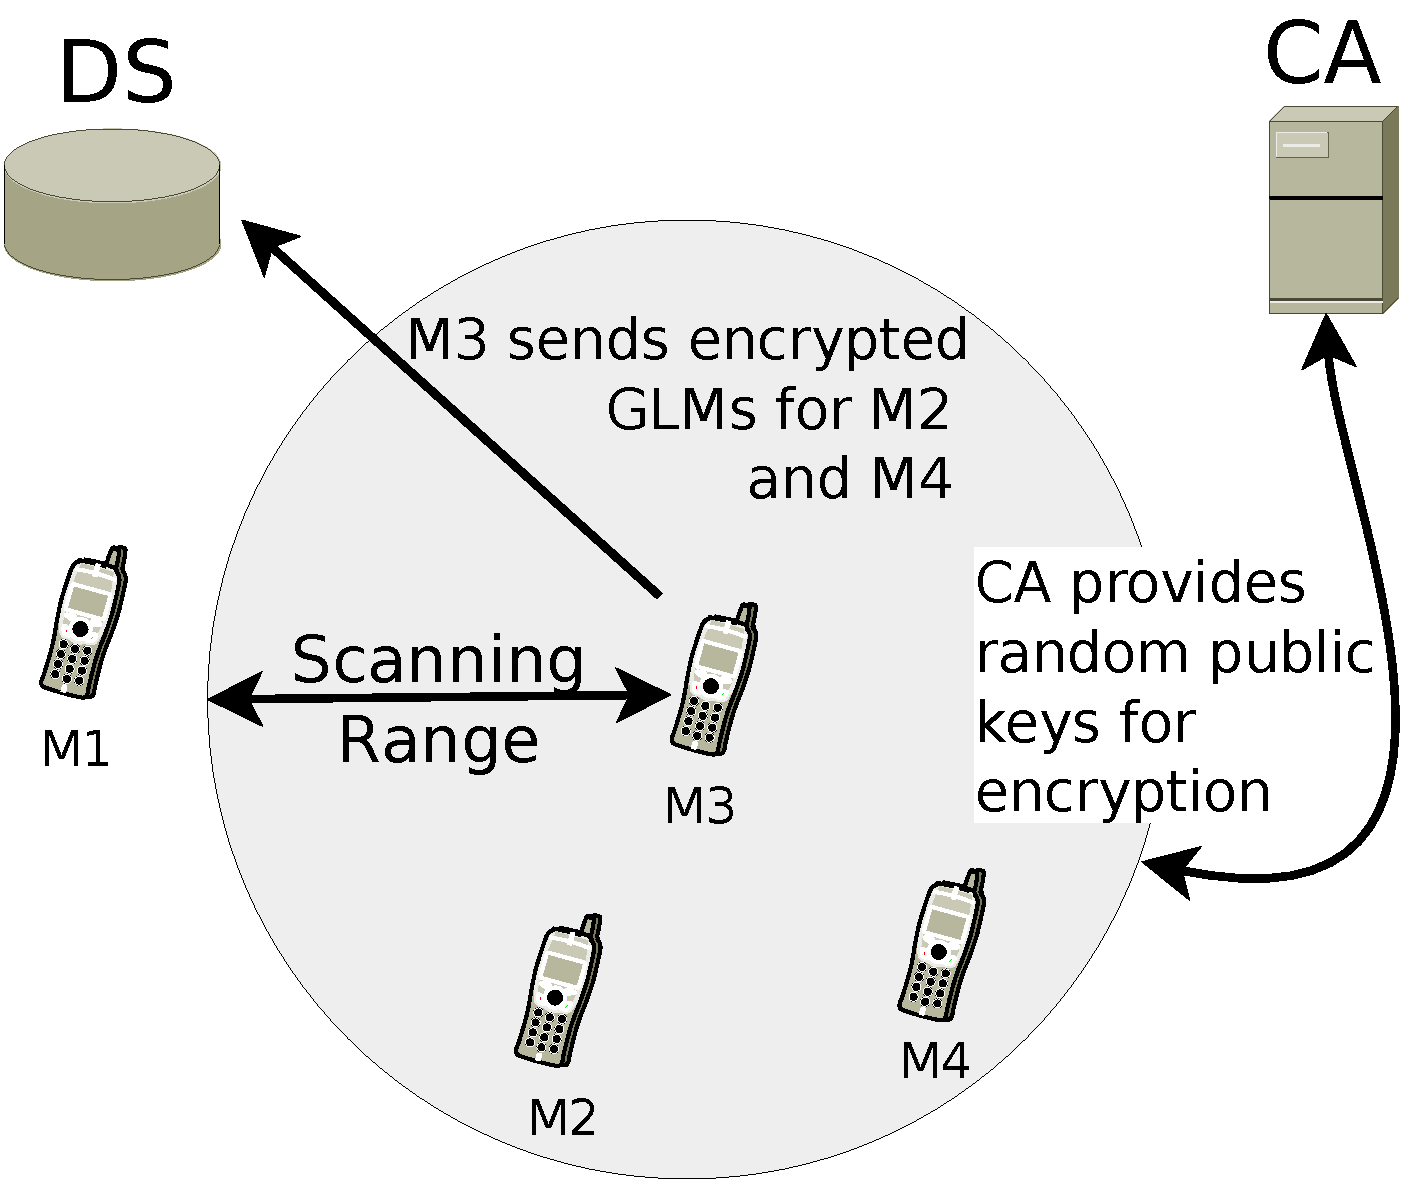
\includegraphics[width=7cm]{diagram/SAT-overview.pdf}}
\caption{\textit{SAT protocol overview. M3 sends an encrypted location report for M2 and M4}}
\label{fig:sat-example}
\end{figure}

In Figure \ref{fig:sat-example} we show an example for the SAT system model. The mobile phone M3 is within range of M2 and M4, therefore M3 will send a GLM for M2 and M4 to the DS. A GLM message includes the sensor nodes' location, the date \& time, a public key identifier and the detected MAC addresses. The public key identifier is needed to be able to decrypt the GLM again using the correct private key. The location data inside the GLM is encrypted using random public keys provided by the CA for privacy preservation. The location information inside the GLM is the only content inside the GLM which is encrypted.

%The goal of the SAT system is to provide a secure privacy preserving distributed tracking system which offers higher tracking accuracies compared to current GSM network based positioning technologies. The SAT system can be used to provide historic or real time tracking.
%The entities for SAT are the mobile phone nodes, the Data Storage Server (DS) and the Certificate Authority (CA).\\


\section{The SAT protocol}
Sensor nodes detect other Wifi enabled devices in their vicinity using Wifi passive scanning. When a message is intercepted the detecting node sends a GLM to the DS which includes the targets MAC address and the detecting node's location. The DS collects and stores the GLMs for later tracking purposes. Each sensor node needs the SAT Application installed and Wifi enabled to be able to intercept surrounding Wifi traffic using passive scanning.\\


%Phone nodes retrieve a public key from the CA which is used to encrypt the GLM positioning reports before sending it to the DS (see Figure \ref{fig:sat-example}).\\

The CA provides the random pseudonym certificates which are used by the mobile phone nodes to encrypt the GLM records. For each GLM record the phone obtains a new random private key from the CA. The encrypted GLMs are sent to the DS which stores all records for later tracking use. \\
\begin{comment}
Each time the scanning phone detects a target it will report the target and send it's own location along with it. The DS collects all reported detections of the tracking target. Using the reported data it is possible to compute the movements of the target without the need of any stationary infrastructure.\\
\end{comment}




\subsection{Target logging}
A node detects all Wifi MAC (BSSID) addresses by passive scanning all Wifi communications every 15 seconds (the ScanningInterval) in its area. The node subsequently sends the detected MAC addresses as a GLM to the DS. A GLM report includes the following information:
\vspace{0.25cm}

\begin{itemize}
 \item 32 bit integer as Latitude (encrypted)
 \item 32 bit integer as Longitude (encrypted)
 \item 46 bit Wifi BSSID MAC address of the target detected
 \item 128 bit integer as public key identifier
 \item 40 bit time stamp
\end{itemize}

\vspace{0.5cm}
Each GLM has its location information encrypted using a new random public key obtained from the CA (see Figure \ref{fig:sat-example}). Since the location information inside the GLM are encrypted the DS cannot use the GLMs for tracking without obtaining the decyption keys for the GLMs.


\subsection{Target tracking}
In order for the LEA to trace a target using SAT, they need to first obtain the target's GLM records and the neccessary decryption keys. This is due to the pseydonym public key infrastructure (PPKI) which is used to encrypt the position locatio inside the GLM. Figure \ref{fig:sat-comm} showcases the required communications for the LEA to track a target. The sensor node detects  another smartphone and fetches a new private key from the CA (Step 1). Subsequently the sensor nodes submit an encrypted GLM to the DS.\\

In order for the LEA to trace a target they first need to obtain the GLM records for the target of interesst (Step 3). Since the location information is encrypted inside the GLM records, the LEA needs to obtain the decryption keys from the CA to be able to decrypt the records and trace the target (Step 4). The LEA then uses the GLM records to track the target's position.\\


\begin{figure}[h]
\centerline{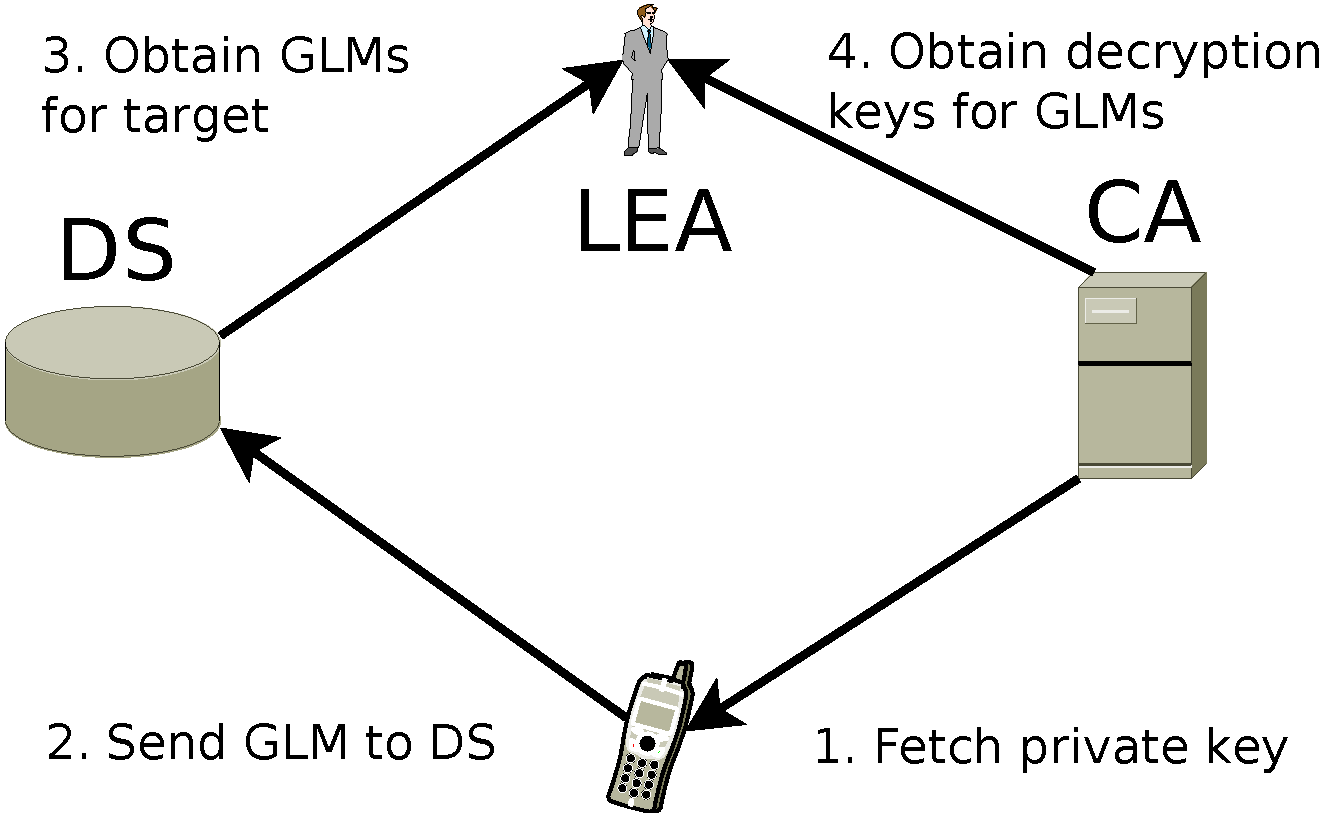
\includegraphics[width=7cm]{diagram/SAT-communication-2.pdf}}
\caption{\textit{SAT protocol communication overview}}
\label{fig:sat-comm}
\end{figure}









%\begin{wrapfigure}{r}{6.5cm}
%  \begin{center}
%    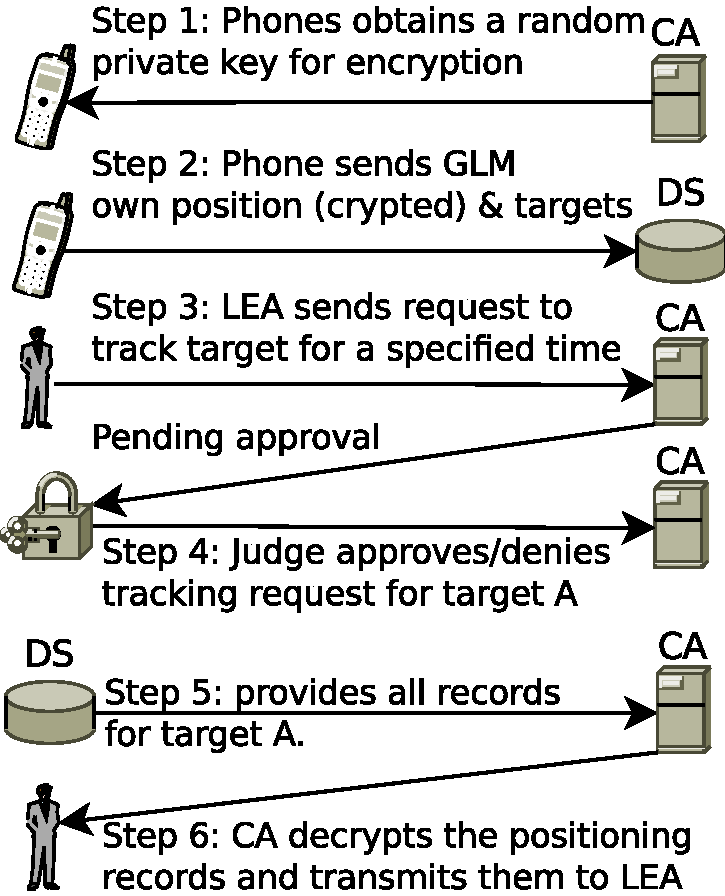
\includegraphics[width=6.5cm]{diagram/SAT-communication.pdf}
%  \end{center}
%  \caption{\textit{SAT communication and Agent interaction}}
%  \label{fig:sat-comm}
%\end{wrapfigure}

%The DS which stores all records is under the control of the LEA. The CA, which provides the
%Public Key Infrastructure (PKI) and decryption, is under the control of the Judges or a trusted 3rd party provider. The encryption together with the anonymous random pseudonym public keys ensure privacy. The division of power between the LEA and the Judges is essential since without this distribution of power there would be no privacy.


This concludes our SAT protocol explanation. If a reader has questions about SAT we would like to refer the reader towards Canlar et al. \cite{SAT} which is the original paper proposing SAT. Canlar's paper explains SAT in greater detail than required in this paper.\\

In summary the SAT protocol offers good privacy protection, requires no stationary infrastructure and is expected to provide better accuracies compared to current GSM network based tracking methods.





\section{Simulation Setup}
%\subsection{Why simulation}
Currently no real world data sets exist that is suited to simulate the SAT protocol \cite{MALNET}. 
Such a data set would require complete and accurate positioning data for every person inside a city inside a 24 hour time frame.\\


We use the UDel Simulator \cite{UDEL} to generate the movements of 9056 people walking inside a 3x3 block area in downtown Chicago. ``The UDel mobility simulator is based on surveys from a number of research areas including time-use studies performed by the US Department of Labor and Statistics, time-use studies by the business research community, pedestrians and vehicle mobility studies by the urban planning and traffic engineering communities. Based on these works, the mobility simulator simulates arrival times at work, lunch time, breaks/errands, pedestrian dynamics (e.g., realistic speed-distance relationship and passing dynamics), and workday time-use such as meeting size, frequency, and duration'' \cite{UDEL}. These characteristics make UDel a good choice to generate the movements inside a city.\\

\begin{comment}
Husted et al.  show that there currently exists no complete and
accurate mobility data set for 100\% or the majority of the population inside a city.
Furthermore they explain that creating such a data set is too expensive. It would require
complete and accurate data about the position of every person inside the town.\\
The only potential candidate would be telco location data. However telco data does not have enough
accuracy and there are legal issues even if the data would be ethically used.
We use the UDel Simulator  \cite{UDEL} to generate mobility data of pedestrians
walking through Chicago. Husted et al. \cite{MALNET} in their research about a malicious scanning network use a similar simulation setup.
\end{comment}



%\subsection{SAT simulation assumptions}
In order to be able to simulate SAT we have to make some assumptions. Most notably we do not simulate any detection success (or failure) rates. If a node is within two dimensional \texttt{Range} of another phone, detection is guaranteed. We use the \texttt{Range} between nodes very precisely. For example if the \texttt{Range} is configured to be at 30m (meters), then there will be no detection if the distance is 30,1m.\\

Our simulations are using 9056 walking pedestrians in a 9 block area from Chicago. Walking pedestrians inside a city are an ideal and realistic environment to conduct our SAT simulation study. Real world radio based connectivity issues are also not simulated as simulating such issues correctly without previous research out of scope for this thesis. All nodes can detect the target if the target is inside the scanning \texttt{Range}. Detection is immediate and guaranteed if the target is within the scanning \texttt{Range}. All witnesses (mobile nodes) are aware of their precise current position. We assume that the target and witness nodes all have Wifi enabled at all times, which is a necessity for the SAT protocol, as detection is based on the Wifi MAC addresses. The target localisation is computed using a two-dimensional centroid like algorithm.\\

%\subsection{UDel mobility parameters}
We use the UDel Simulator Version 1 \cite{UDEL} and a 9 block area of Chicago to generate 24 hours of mobility data with 9056 walking pedestrians. The maximum walking speed of the pedestrians is 1,79 meters per second, the minimum walking speed is 0,70 meters per second, which are the default settings for the UDel simulator. The generated mobility data is then used as input to conduct our simulations using our own written SAT simulator.\\



%\subsection{Simulation parameters}
The SAT simulation was developed with the following input parameters which have an influence on the outcome:\\

\begin{itemize}
 \item \texttt{ScanningInterval}: How often do nodes scan for other nodes (seconds).
 \item \texttt{Delta}: All reports within a \texttt{Delta} time frame are aggregated, and a target triangulation is computed from all reports which are inside the \texttt{Delta} timeframe (seconds).
 \item \texttt{Range}: This is the detection range of nodes. If another node is within this Range it will be discovered (meters).
 \item Another input to our SAT simulator is the UDel mobility file, which contains all the movement data of the whole population.
\end{itemize}

\vspace{0.5cm} These are the values which we used to conduct our simulations. For \texttt{ScanningInterval} we used \{1, 15, 30, 60\} seconds. For \texttt{Delta} variable we used 30 and 60 seconds. Furthermore for \texttt{Range} we use \{15, 30, 45\} meters. All combinations of the above settings are simulated and aggregated into our resulting data, which
means that only \textit{one} variable will change and all other simulation results are combined and shown. This gives the best overview on how  a specific variable influences the tracking results. For all simulations we used a minimum of 3 witnesses to compute a triangulation. If there were only 2 witnesses reporting the target during a given \texttt{Delta} interval, then no triangulation is computed and the \texttt{Delta} interval is skipped creating a (small) tracking gap.\\

\begin{algorithm}
\caption{Triangulation algorithm used during our simulations.\newline Averaging witness pairs, then average those to compute the final positioning}\label{sat-triag}
\label{alg:triag}
\begin{algorithmic}[1]
\Procedure{Triangulate}{$witnesses$}
\State $n \gets 0$ \Comment{Initialise variables}
\State $x \gets 0$
\State $y \gets 0$
\For{$i \gets 0 \textrm{ to } (witnesses.size()-1)$}
\For{$j \gets 0 \textrm{ to } (witnesses.size()-1)$}
\If{$i \not= j$} \Comment{Continue only with 2 \textit{distinct} witnesses}
  \State $x \gets x + ((witnesses.get(i).getX() + witnesses.get(j).getX()) / 2)$
  \State $y \gets y + ((witnesses.get(i).getY() + witnesses.get(j).getY()) / 2)$
  \State $n \gets n + 1$
\EndIf
\EndFor
\EndFor
\State $x \gets x / n$ \Comment{Compute the average of the temporary Data}
\State $y \gets y / n$\\
\Return $(x , y)$


\EndProcedure
\end{algorithmic}
\end{algorithm}


%\subsection{Simulation runs}
For each configuration we run 10 simulations on 10 different targets to ensure we receive a balanced set of results. Each simulation is a 24 hour simulation in which a specified target gets traced using our SAT protocol. As detection network we use 10\% of the total population (9056). For each simulation run we pick a \textit{random} 10\% subset from the total population of nodes. The selected nodes act as distributed detection network to simulate the SAT protocol.\\

From each 24 hour simulation we compute the average and standard deviation from all tracking/triangulation results. This gives us 10 average and 10 standard deviation values for each simulation configuration. The 10 values are then averaged to receive the final values shown in the graphs (Figure 2-5).\\

%move this to simulation results?



We use one algorithm to compute the target position from the witness reports. This algorithm is often referred to as Centroid. Though the Centroid only averages the witness positions once. We took a slightly different approach since we average the positions twice. In Algorithm \ref{alg:triag} we take the position average of each witness \textit{distinct} pair (lines 5 -- 13). Then as a last step we compute the average again to obtain the triangulation end result (lines 14 -- 16).\\







\section{Simulation results}
\subsection{Tracking accuracy results}
The \texttt{Delta} variable is the time interval which is used to aggregate witness reports to compute the location of a tracked target. In other words it could also be called a Positioning Interval, because in these time intervals the target's position is calculated.\\

The \texttt{Delta} variable, for which we used 30 and 60 seconds in our simulations, has no influence on the tracking deviation results. For both \texttt{Delta} values the mean tracking deviation is 9.7 meters. This is the mean deviation from the target's actual (real) position. It is important to note that in our simulations tracking gaps \textit{do not} negatively impact the mean tracking deviation. To give an exaggerated example: if during 24 hours a target was only traced once with a deviation of 10 meters, then the mean tracking deviation will show 10 meters as well. This is because whenever a tracking gap occurs there is no accuracy penalty. Additionally since we simulate slow moving pedestrians, the \texttt{Delta} has a smaller impact than if we simulated faster moving objects in our SAT simulations. For example if we simulated faster moving cars, then a \texttt{Delta} of 30 seconds would result in higher accuracies compared to a \texttt{Delta} of 60 seconds. This is because a car moves over a longer distance in 60 seconds compared to 30 seconds.\\

\begin{figure}[t]
\begin{minipage}[b]{0.45\linewidth}
\centering
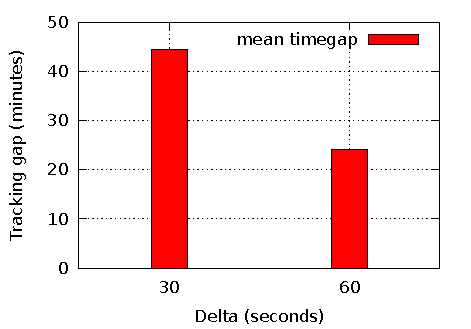
\includegraphics[width=7cm]{delta-timegap-total.pdf}
\caption{\textit{Delta variable and average tracking gaps}}
\label{fig:delta-timegap-deviation}
\end{minipage}
\hspace{0.5cm}
\begin{minipage}[b]{0.45\linewidth}
\centering
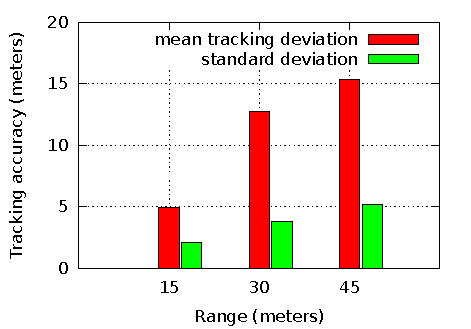
\includegraphics[width=7cm]{range-deviation-total.pdf}
\caption{\textit{Range variable and tracking accuracy}}
\label{fig:range-deviation}

\end{minipage}
\end{figure}

A higher \texttt{Delta} value decreases the tracking gaps (Figure \ref{fig:delta-timegap-deviation}). For each \texttt{Delta} time interval we aggregate all witness reports together to compute the target's location. If for a given \texttt{Delta} interval there are less than 3 witnesses, then no triangulation is computed and the \texttt{Delta} interval is skipped. Since increasing the \texttt{Delta} variable essentially requires less witness reports per minute, the reduced amount of tracking gaps using a \texttt{Delta} value of 60 seconds was to be expected compared to the lower \texttt{Delta} value of 30 seconds.\\


The \texttt{Range} variable in our simulation defines the scanning range of a sensor node. Our simulator uses the \texttt{Range} variable as a hard cutoff between detection and non detection. Pedestrians move slowly, so a \texttt{Range} of 15 meters will resulting in an accuracy of at least 15 meters. In our simulations we use the \texttt{Range} variable very accurately, which means that if a node is at a distance of 15,1 meters using \texttt{Range} 15 meters, then no detection occurs.\\

The \texttt{Range} variable has a direct impact on the tracking accuracy (Figure \ref{fig:range-deviation}). The higher the \texttt{Range} the higher is the tracking deviation from the target's actual location. This is quite clear since we use the \texttt{Range} variable so strictly in our simulations.\\

A higher \texttt{Range} decreases the tracking gaps since with increased range the amount of GLMs sent increase as well. The more witness reports are available in a given \texttt{Delta} period the fewer tracking gaps will occur.\\


A \texttt{ScanningInterval} of 60 seconds reduces the tracking gaps (Figure \ref{fig:scanninginterval-timegap}). A tracking gap is the biggest gap between two computed target positions. A \texttt{Delta} of 60 reduces the tracking gaps, since it allows for more witness accounts to be used for each positioning interval. If for any given \texttt{Delta} there are 2 or less witness reports, the data is discarded and no triangulation is computed. This makes it possible for the tracking gaps to exist. The tracking gaps are at night when the simulated population is ``at home''. The UDel Model simulator simulates the typical urban commuting traffic. Which means during the day, due to the increased population amount inside the city, there are fewer tracking gaps.\\


%A higher \texttt{ScanningInterval} means we have less witness reports for a given \texttt{Delta}. For a valid triangulation we require at least three witnesses, if only 2 witnesses observed the target during a \texttt{Delta} interval the positioning data is discarded. An algorithm that is flexible towards the amount of witness reports can use more advanced heuristics to adapt between many reports and very few witness reports.\\

The \texttt{ScanningInterval} is the time interval that the sensor nodes use to scan for other Wifi enabled devices. A higher \texttt{ScanningInterval} means less detection attempts per minute, so it does not come as a surprise that a higher \texttt{ScanningInterval} value increases the tracking gaps (Figure \ref{fig:scanninginterval-timegap}). The \texttt{ScanningInterval} setting has a direct influence on the amount of GLMs that are being reported, which influences these tracking gaps. These tracking gaps occur in our simulations at night time, when the lowest population amount is inside our simulated area. A \texttt{ScanningInterval} of 1 second provides the most witness reports (GLMs), which allows for the highest traceability with a minimum amount of tracking gaps (see Figure \ref{fig:scanninginterval-timegap}). However the bandwidth requirements using \texttt{ScanningInterval} of 1 are high, needing about 40 mbit of bandwidth in our simulations.\\

The \texttt{ScanningInterval} has no influence on the mean tracking deviation. Like we elaborated earlier this is due to the fact that, if no triangulation could be computed during a \texttt{Delta} interval, there is no accuracy penalty applied. This means that all triangulations that have been computed have the same degree of accuracy , regardless of the actual \texttt{ScanningInterval} used. Since we only compute the deviations between actual triangulations, the tracking deviation results do \textit{not} reflect or include tracking gaps in any way.




%if someone is moving in a train, a 60 second \texttt{Delta} would be enough to see huge location tracking deviations from actual position.












\begin{figure}[htb]
\begin{minipage}[b]{0.45\linewidth}
\centering
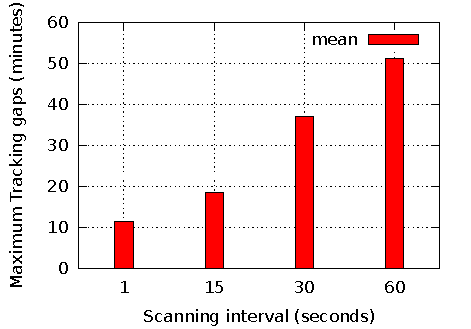
\includegraphics[width=7cm]{scanninginterval-timegap-total.pdf}
\caption{\textit{ScanningInterval variable and average tracking gaps}}
\label{fig:scanninginterval-timegap}
\end{minipage}
\hspace{0.5cm}
\begin{minipage}[b]{0.45\linewidth}
\centering
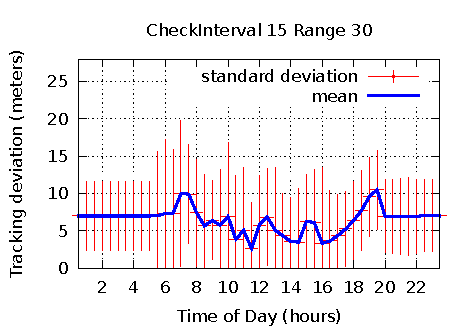
\includegraphics[width=7cm]{24-deviation-view.pdf}
\caption{\textit{24 hour tracking accuracy overview using ScanningInterval 15 Range 30 as configuration}}
\label{fig:24h-detail-view}

\end{minipage}
\end{figure}

The potential tracking accuracies of SAT protocol can be seen in Figure \ref{fig:24h-detail-view}. In our simulation the sensing smartphones are aware of their precise own location. Cheng et al. \cite{CHENG} showed that smartphones can use Wifi alone to determine their own position with an average accuracy of 25 meters in urban environments. As you can see in Figure \ref{fig:24h-detail-view} the configuration shown has an accuracy of under 10 meters. If we add another 20-30 meters deviation from
the smartphone self-positioning, the potential SAT accuracies are likely 50 meters or better most of the time.




\subsection{Bandwidth requirements}
In this section we discuss the the bandwidth requirements of the SAT protocol. The biggest influence on bandwidth usage is the \texttt{ScanningInterval} variable. It directly relates to how many reports are sent to the DS and how much outgoing bandwidth is used by the SAT protocol. A GLM report sent by a node to the DS contains a total payload of 288 bits per message (see Section 3), excluding encryption.\\

The location information of the payload data is encrypted using the public key obtained from the CA and the actual payload size increases. Using Eliptic Curve Cryptography (ECC) together with 1024 bit keys results in a netto payload of 9 kilobytes after the GPS coordinates have been encrypted. The 9 kilobytes already include a 10\% added overhead to account for TCP/IP overhead.



\begin{figure}[ht]
\begin{minipage}[b]{0.45\linewidth}
\centering
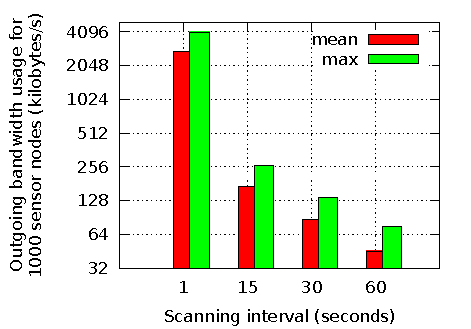
\includegraphics[width=7cm]{scanninginterval-bandwidth-total.pdf}
\caption{\textit{Bandwidth usage in kilobytes per second and scanning interval. The data shown is for 1000 sensor nodes.\\Note: the Y-Axis uses log scaling.}}
\label{fig:bandwidth-view}
\end{minipage}
\hspace{0.5cm}
\begin{minipage}[b]{0.45\linewidth}
\centering
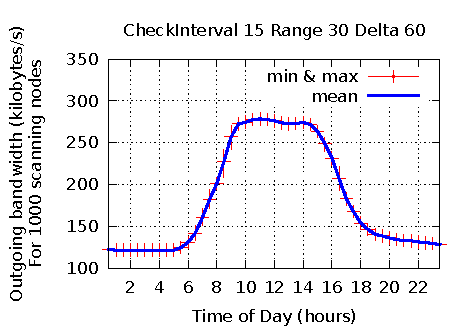
\includegraphics[width=7cm]{24-bandwidth-view.pdf}
\caption{\textit{24 hour bandwidth overview using Delta 60 ScanningInterval 15 Range 30 as configuration. The daily commute is visible, busiest time between 8 am and 4 pm}}
\label{fig:24h-bandwidth-view}

\end{minipage}
\end{figure}
\vspace{0.5cm}

If phones are configured to detect every other communication device for \textit{every second}
the simulations show that the SAT protocol requires 40 megabit of outgoing bandwidth for 1000 sensor nodes (see Figure \ref{fig:bandwidth-view}). Detecting every Wifi device in the vicinity within 1 second intervals is not desirable, not only due to the high bandwidth requirements. The power consumption would be higher compared to higher \texttt{ScanningIntervals}, like 15 seconds or higher.\\

The bandwidth requirements for a \texttt{Scanning Interval} of 15 seconds are 15 times less requiring only 3 mbit in comparison. This significant difference (40 mbit vs 3 mbit) makes the \texttt{Scanning Interval} of 15 seconds interesting. In Figure \ref{fig:24h-bandwidth-view} we show the bandwidth for 24hours using 15 seconds as \texttt{Scanning Interval}. The daily commute into and out of the city is clearly visible, with more bandwidth used mid-day.\\

The SAT bandwidth requirements for configurations using \texttt{ScanningInterval} of 15 or higher are moderate, requiring less than 3 mbit of outgoing bandwidth per 1000 scanning nodes. It is our opinion that such bandwidth usage is already tolerable for current mobile phone networks, keeping in mind that the bandwidth capacity of mobile internet are steadily increasing due to high demand.


The SAT protocol traces a phone (device) with less than 15 meters accuracy in 30 seconds intervals. In 24 hours the SAT trace has a maximum average tracking gap of 10 minutes in an ideal simulated environment. Our simulations show that the results are all linearly connected. There is no threshold which drastically changes the results when reached. The opposite is true, the results degrade linearly if the configuration settings are changed towards less ideal settings.

%state how much BW is needed. not that there is a possibility




%Gruteser et al. \cite{GRUTESER} propose disposable MAC addresses, a randomization feature
%which would counteract tracking networks such as the Sense-And-Trace protocol. This increases the privacy of Wifi users
%because it randomizes the normally static MAC addresses which get sent over the air in plain text. In \cite{GREENSTEIN} researchers propose
%a protocol which eliminates the use plain text MAC identifiers using a combination of cryptographic methods and
%obfuscation, increasing privacy. This would also counteract our proposed SAT protocol as it relies on the Wifi identifier (MAC)
%to identify the tracing target.

\begin{comment}
\subsection{Privacy preservation}
There currently is no metric indicator representing privacy.
\textit{Wong et al} \cite{WONG} suggest that ``\textit{Anonymity of a system
may be defined as the amount of information the attacker is missing to
uniquely identify an actor's link to an action}''. Using this as a metric,
while not a comparable numeric metric, the  SAT protcol can be considered as very privacy
preserving. The operator of the DS (i.e. the government) only get's random certificate key id's
for each witness report received. Since these are randomized the operator/government has only
the certificate id and a location from the witness node. 
\end{comment}

\section{Feasibility \& open problems}
In this section we present challenges that a real world implementation of our SAT protocol would face.\\

\textbf{MAC address randomisation}. The biggest issue is that the SAT protocol is designed to detect Wifi communications using the Wifi MAC address (BSSID) as unique identifier. This MAC address is static on current devices making it a suitable unique identifier for tracking. However the reliance of SAT on Wifi MAC addresses, make it vulnerable to MAC address randomisation or other techniques which prevent the MAC address from being sent over the air in plain.\\
Wifi protocol improvements have been proposed by Greenstein et al. \cite{GREENSTEIN} and Gruteser et al. \cite{GRUTESER} which would both directly counteract the SAT protocol by masking the MAC address, preventing it from getting sent in plain over the air. A user could also just change their Wifi MAC identifier and throw off the distributed SAT sensing network. As last resort the LEA can plant a probe which emits Wifi beacons to use for tracking if the tracked target changes their MAC address.\\

\textbf{Listening on multiple frequencies at once}. Current smartphones while powerful and versatile are unable to listen to all common Wifi channels at once. As such Wifi probing requests could be missed. If there is steady traffic flow between the target Wifi device and an AP then detection, if within reception range, is guaranteed. Canlar et al \cite{SAT} state that scanning takes 550 milliseconds per channel, giving a total scanning time of just over 6 seconds.\\
We are unsure if Wifi devices looking for Wifi networks will send beacon requests at high interval to give a high chance of detection. Since a node would be only listening 550 milliseconds per channel it is unclear how high the chances are for detection. Further research needs to be done to find out how many beacon requests an idle Wifi device sends.
The 801.11 standard \cite{80211} on page 421 explain that Wifi probes get sent less when other Wifi devices send probes.


 A low level hardware approach needs to be taken to really find out how high the probability is that a scanning node detects another node during the 550 millisecond passive scan window.\\
For our simulation we assumed that detection is guaranteed if within range, however this assumption may not hold true in the real world. Hence why we suggest to research this on a hardware level to find out how likely detection is given close proximity.\\

\textbf{Battery Life}. Until battery capacity increases significantly it can be hard to convince users to install an App to become part of the distributed sensing network. Due to restricted battery life on smartphones at the moment it would be hard to convince users to install the SAT application even with good incentives, as proposed in \cite{SAT} and \cite{MALNET}. Technical users may be reluctant to install such an App due to the potential battery drain it can cause.\\
A hardware implementation on smartphones could force everyone to become part of the SAT network.\\

\textbf{Intercepting Wifi channels}. It is not clear if every mobile phone has the capability to \textit{monitor} Wifi channels. For example we tried monitoring using a laptop running Ubuntu 12.04, however either the Wifi chip or its drivers prevented us from monitoring surrounding Wifi traffic.\\

\textbf{Distribution of power}. The privacy preserving aspects of SAT lie in the way the data
and the witnesses are protected. While the security and privacy do not play
a huge role in this paper it is an important design goal of SAT and deserves some explanation.\\
The location data inside the GLMs are encrypted using the random private key fetched. This encryption
protects the witnesses privacy, ensuring the LEA cannot trace everyone since they would require the decryption keys.\\
The CA on the other hand has the decryption keys, which makes it important that the DS and the CA
are controlled by 2 independent parties, to divide the power. The DS which contains the encrypted data are controlled by the LEA. The Judicary(Judges) control the SAT smartphone app implementation, and the CA infrastructure. Judges themselves won't be able to maintain it, but an independent employee who works on behalf of the judges and works in their interest has to maintain the CA.\\
It is important that the Judges (CA) and LEA (DS) do not conspire together, as this would effectively reveal the location from everyone, witnesses and targets alike. The boundaries of the LEA and CA have to be strictly adhered to, in the implementation, as otherwise there would be no privacy.\\
So as can be seen in Figure \ref{fig:sat-example}, the Judges literally hold the key (and the cryptographic keys too) to allow or deny the LEA's tracking requests. The LEA cannot use the data on the DS without the decryption keys, for which they need the Judges approval. This division of power using cryptographic protections gives SAT its privacy preserving qualities. If the division of power is not correctly implemented, then there is no privacy at all, so correct implementation is crucial.\\

\begin{comment}
\subsection{Privacy preservation}
However Multy Hypothesis Tracking as researched by Wiedersheim et al \cite{WIEDERSHEIM}
is a potential risk for the privacy preserving properties of the SAT protocol.
Wiedersheim's research and simulation was done in the context of cars, so their results may not
be comparable to a condensed amount of phones. The SAT protocol works best in a populated urban
environment. We leave this as future work for other researchers to investigate.
\end{comment}

\section{Conclusion}
The SAT protocol is a distributed tracking network alternative offering higher accuracies compared to GSM network based localisation tracking. Our simulation study shows that in an ideal simulated environment SAT can offer accuracies of under 15 meters. Smartphones have a self-positioning deviation of 25 meters on average, and even if we add the self-positioning deviation in full the SAT protocol will show accuracies of 40 meters or better.\\
The bandwidth requirements of SAT are reasonable, using less than 3 mbit per 1000 scanning nodes. Today's mobile phone networks should be able to cope with such a bandwidth consumption. As the mobile phone networks improve their capacities, in future a deployment of SAT will not significantly impact the mobile phone networks. Video or other media usage patters will consume a lot more bandwidth in comparison.\\
The feasibility of implementing SAT in a real-world scenario is unclear, even after our work. The implementation itself is not the concern. It is however unclear how high the detection chances are given close proximity of two smartphones. If both have Wifi enabled and one of the two smartphones has the SAT application installed and running, how likely is it that SAT detects the other smartphone? A Wifi enabled device, which is currently not logged into an AP may not send beacons fast enough for SAT to have a high chance of detection the other smartphone's Wifi communications. We suggest for further research to be done to find out how likely detection is on a low level hardware point of view.\\
The accuracies which SAT can offer are very interesting mainly because SAT relies on short range radio frequency detection (Wifi). GSM networks on the other hand have a higher communication range which makes it harder for them to compute a highly accurate position for a phone. The communication range of GSM is higher than the Wifi communication range, which makes Wifi the more suitable technology for positioning. Wifi-self positioning is a good example for this, achieving accuracies of 25 meters. If the same self-positioning technique were usable for GSM, the accuracies would be worse due to the increased communication range and reduced amount of Base Stations available compared to Wifi.





% include bibtex bibliography

%\newpage
%\bibliographystyle{acm}
\newpage

\bibliographystyle{siam}
{\footnotesize\bibliography{references.bib}}


\begin{comment}
\section*{Appendix}
A picture showing the 9x9 block area in Chicago modeled by the Udel Model simulator.
The map and picture are from the UDel website \cite{UDEL}.

\begin{Figure}[h]
\centering
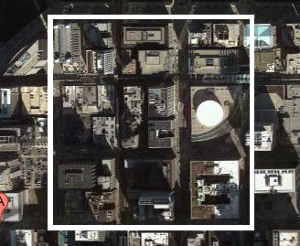
\includegraphics[width=8cm]{chicago-3x3-block-map-radar.png}
\caption{\textit{Satelite image of 3x3 block area simulated in UDel}}
\label{fig:delta-timegap}
\end{Figure}

\begin{Figure}[h]
\centering
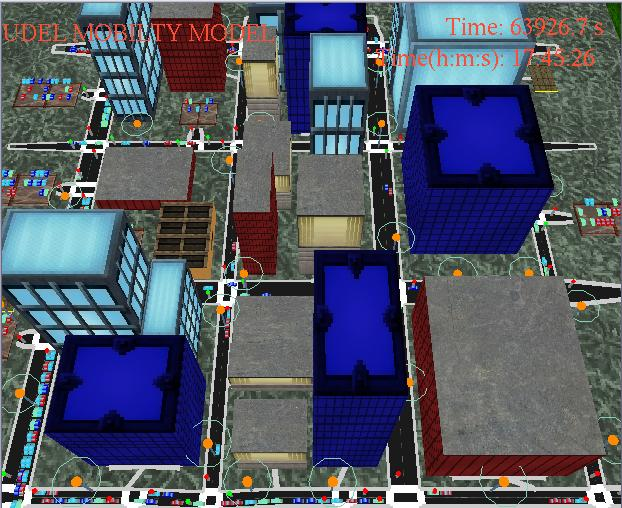
\includegraphics[width=8cm]{Chicago9x9Blk.jpg}
\caption{\textit{UDel model of 3x3 block area in Chicago}}
\label{fig:delta-timegap}
\end{Figure}
\end{comment}

\end{document}
